\chapter{Blasting, Fast and Slow} 
\lstset{style=6502Style}

Every game has a 'main loop'. A tight section of code which is executed multiple times
per second and which controls nearly all aspect of the gameplay. In Iridis Alpha this
boiler-room is \icode{PerformMainGameUpdate}:

\begin{lstlisting}[caption=\icode{PerformMainGameUpdate}\, the spaghetti junction handling nearly everything
during main gameplay.]
;-------------------------------------------------------
; PerformMainGameUpdate
;-------------------------------------------------------
PerformMainGameUpdate
        LDX currentPlanetBackgroundClr1
        LDA backgroundColorsForPlanets,X
        STA $D022    ;Background Color 1, Multi-Color Register 0
        LDX currentPlanetBackgroundClr2
        LDA backgroundColorsForPlanets,X
        STA $D023    ;Background Color 2, Multi-Color Register 1

        LDA $D01F    ;Sprite to Background Collision Detect
        STA spriteCollidedWithBackground

        JSR CheckKeyboardInGame
        JSR ScrollStarfieldAndThenPlanets
        JSR AnimateGilbySpriteMovement
        JSR PerformMainGameProcessing
        JSR CheckForLandscapeCollisionAndWarpThenProcessJoystickInput
        JSR CalculateGilbyVerticalPositionEarthBound
        JSR CalculateGilbyVerticalPositionAirborne
        JSR MaybeDrawLevelEntrySequence
        JSR PlaySoundEffects
        JSR FlashBorderAndBackground
        JSR UpdateGilbyPositionAndColor
        JSR UpdateAndAnimateAttackShips
        JSR UpdateBulletPositions
        JSR DrawUpperPlanetAttackShips
        JSR UpdateControlPanelColors
        ; Jump into KERNAL's standard interrupt service routine to 
        ; handle keyboard scan, cursor display etc.
        JMP ReEnterInterrupt 
        ;Returns From Interrupt
\end{lstlisting}

Just like in the title sequence this routine is called dozens of times as the 
beam of light painting the screen travels from top to bottom up to 25 times per second.
\icode{PerformMainGameUpdate}, along with a routine called \icode{AnimateStarFieldAndScrollPlanets}
whose purpose you can hopefully guess from its name, are the two gears that grind out the
gameplay as long as the player is alive and blasting. 

\afterpage{%
  \begin{figure}[H]
      \centering
      \foreach \l in {0,...,299}
      {
        \includegraphics[width=1cm]{main_game/one_second/main\l.png}%
      }%
  \caption{The screens displayed in a single second of game time.}
  \end{figure}
  \clearpage
}

For each pass through the screen \icode{AnimateStarFieldAndScrollPlanets} is executed 8 times
while \icode{PerformMainGameUpdate} is executed once.

\begin{figure}[H]
    \centering
    \foreach \l in {5368,...,5378}
    {
      \includegraphics[width=3cm]{main_game/main_loop/main\l.png}%
    }%
\caption{The rasterline positiion when \icode{AnimateStarFieldAndScrollPlanets} and \icode{PerformMainGameUpdate} are called.}
\end{figure}

If you look closely you'll notice that our so-called boiler-room routine is called last, when the
raster is nearing the end of the screen. This makes sense as it has the most to do and therefore
we need to execute it at a point when most of the screen has been painted and what to paint on the
rest of it has already been prepared. \icode{PerformMainGameUpdate} primarily concerns itself with
preparing the screen for the next time it will be painted: updating the position of the enemies
on the upper planet, the position of the player's ship, playing sound effects, moving the bullets
and so on. 

\icode{AnimateStarFieldAndScrollPlanets} on the other hand only has to worry about painting the 
parallax starfield in the background, scrolling the planets using the C64's specialized hardware,
and preparing the position of the enemy sprites on the lower planet. The only reason it is called
more than once is because, like in the title screen routine, the starfield is being painted using
a single sprite (Sprite 7). Each time it runs it can change the position of this sprite so that
it appears at a new position as well as the old one on which the raster has already painted it. We
covered the mechanics of this in detail when we dissected the title screen in 'The First 16 Milliseconds'.

\subsection{Updating Enemy Sprite Positions}
We can get a better sense of how the labour is divided between the two routines if we isolate the
position of the raster when the position of the enemy sprites on each planet is updated.

\begin{figure}[H]
    \centering
    \foreach \l in {987,...,988}
    {
      \includegraphics[width=6cm]{main_game/attack_ships/attack_ships\l.png}%
    }%
\caption{The rasterline position when the enemies on the upper and lower planets are updated.}
\end{figure}

The routines for updating the sprites on the upper and lower planets are identical. If we were writing
this game in any other language than assembly we would just have one function and pass the different
arrays for each planet in as parameters. 

\begin{minipage}[b]{0.55\linewidth}
\centering
\begin{lstlisting}[basicstyle=\tiny]
DrawUpperPlanetAttackShips
        LDX #$0C
        LDY #$06
UpperPlanetShipsLoop   
        LDA upperPlanetAttackShipsXPosArray,Y
        STA $D000,X  ;Sprite 0 X Pos

        LDA attackShipsXPosArray - $01,Y
        AND $D010    ;Sprites 0-7 MSB of X coordinate
        STA currentMSBXPosOffset

        LDA upperPlanetAttackShipsMSBXPosArray,Y
        AND attackShipsMSBXPosOffsetArray,Y
        ORA currentMSBXPosOffset
        STA $D010    ;Sprites 0-7 MSB of X coordinate

        ; The X-Pos of sprites is fiddly. The MSB manages
        ; which side of the 512 possible x positions they
        ; are on.
        LDA upperPlanetAttackShipsYPosArray,Y
        STA $D001,X  ;Sprite 0 Y Pos
        STX tempVarStorage

        LDX upperPlanetAttackShipsColorArray,Y
        LDA colorsForAttackShips,X
        STA $D027,Y  ;Sprite 0 Color

        LDA upperPlanetAttackShipsSpriteValueArray,Y
        STA Sprite0Ptr,Y
        LDX tempVarStorage

        DEX
        DEX
        DEY
        BNE UpperPlanetShipsLoop
        RTS
\end{lstlisting}
\end{minipage}
\hspace{0.5cm}
\begin{minipage}[b]{0.55\linewidth}
\centering
\begin{lstlisting}[basicstyle=\tiny]
DrawLowerPlanetAttackShips
        LDX #$0C
        LDY #$06
LowerPlanetShipsLoop   
        LDA lowerPlanetAttackShipsXPosArray + $01,Y
        STA $D000,X  ;Sprite 0 X Pos

        LDA attackShipsXPosArray - $01,Y
        AND $D010    ;Sprites 0-7 MSB of X coordinate
        STA currentMSBXPosOffset

        ; The X-Pos of sprites is fiddly. The MSB manages
        ; which side of the 512 possible x positions they
        ; are on.
        LDA lowerPlanetGilbyBulletMSBXPosValue,Y
        AND attackShipsMSBXPosOffsetArray,Y
        ORA currentMSBXPosOffset
        STA $D010    ;Sprites 0-7 MSB of X coordinate

        LDA lowerPlanetAttackShipsYPosArray,Y
        STA $D001,X  ;Sprite 0 Y Pos
        STX tempVarStorage

        LDX lowerPlanetAttackShipsColorArray,Y
        LDA colorsForAttackShips,X
        STA $D027,Y  ;Sprite 0 Color

        LDA lowerPlanetAttackShipsSpriteValueArray,Y
        STA Sprite0Ptr,Y
        LDX tempVarStorage

        DEX
        DEX
        DEY
        BNE LowerPlanetShipsLoop
        RTS
\end{lstlisting}
\end{minipage}

\subsection{Scrolling the Planets}
We want scrolling to be smooth and fast. Moving swiftly or slowly across the planet surface
depending on how much acceleration we apply is the fundamental dynamic of the game so will
be important to get right.

Exerting some fine-grained control on the scrolling requires us to balance
two fundamental operations: a pixel-by-pixel scrolling mechanism that preserves the smoothness
of movement we want at slower speeds, and a bigger, blunter implement that will accelerate
us across larger sections of the planet while preserving an illusion of relative fluidity.

The first is available as a hardware implementation on the C64. The value stored in the last
three bits of \icode{\$D016} allows us to specify a pixel offset for the planet graphics between
0 and 7, effectively shifting the planet left or right by one or more pixels.

The second is up to us. We need to keep an eye on the speed of our gilby and decide if we should
shift the landscape by one or more full characters.

Here are both of these tactics in operation during two paints of the screen while we're
warping into the Sheep planet at the start of a new game. Each row represents
a single pass of the raster. As you can see we adjust the pixel position using \icode{\$D016}
twice on each pass and adjust the character position once. 

\begin{figure}[H]
    \centering
    \foreach \l in {482,...,487}
    {
      \includegraphics[width=4cm]{main_game/scroll/scroll\l.png}%
    }%
\end{figure}

Since we're moving fairly fast, we're updating the character position by 3 characters on each
occasion (notice how much the bush moves). At the same time we're applying a pixel movement
to preserve the impression of smoothness.

\subsubsection{Pixel Movement}
If we look at the code that looks after the pixel-grained movement in \icode{AnimateStarFieldAndScrollPlanets}
we can see it is using a variable called \icode{planetScrollSpeed} to control the amount of offset to apply:

\begin{lstlisting}[]
        ; Scroll the planet
        LDA $D016    ;VIC Control Register 2
        AND #$F0
        ORA planetScrollSpeed
        ORA #$10
        STA $D016    ;VIC Control Register 2
\end{lstlisting}

This parameter is always kept to a value between 0 and 7, for example here in \icode{DrawPlanetScroll} where it
gets clamped to the last 3 bits (Bits 0 to 2) by an \icode{AND} operation:

\begin{lstlisting}
        LDA planetScrollSpeed
        AND #$07
        STA planetScrollSpeed
\end{lstlisting}

\begin{figure}[H]
  {
    \setlength{\tabcolsep}{3.0pt}
    \setlength\cmidrulewidth{\heavyrulewidth} % Make cmidrule = 
    \begin{adjustbox}{width=6cm,center}

      \begin{tabular}{rllllllll}
        \toprule
        Byte & Bit 7 & Bit 6 & Bit 5 & Bit 4 & Bit 3 & Bit 2 & Bit 1 & Bit 0        \\
        \midrule
        \$FC & 1 & 1 & 1 & 1 & 1 & 1 & 0 & 0 \\
        \$07 & 0 & 0 & 0 & 0 & 0 & 1 & 1 & 1 \\
        \midrule
        Result: \$04 & 0 & 0 & 0 & 0 & 0 & 1 & 0 & 0 \\
        \addlinespace
        \bottomrule
      \end{tabular}

    \end{adjustbox}

  }\caption*{AND'ing a notional value of \$FC with \$07 gives \$04.}
\end{figure}

As you might guess, \icode{planetScrollSpeed} is controlled by the speed of the gilby itself:

\begin{lstlisting}
        LDA planetScrollSpeed
        CLC
        ADC currentGilbySpeed
        STA planetScrollSpeed
\end{lstlisting}

The more we push on the joystick left or right the greater \icode{currentGilbySpeed} becomes. The
greater \icode{currentGilbySpeed} becomes, the more we add to \icode{planetScrollSpeed}. The only
thing we have to be careful about when using this simple mechanic is to ensure that when we update
\icode{\$D016} with \icode{planetScrollSpeed} we are only updating the lower 3 bits - writing to the
rest of them will break things as they are not concerned with scrolling at all. This is why, when
we first retrieve \icode{\$D016} to the \icode{A} register we mask out the first four bits:

\begin{lstlisting}[]
        ; Scroll the planet
        LDA $D016    ;VIC Control Register 2
        AND #$F0
\end{lstlisting}


\begin{figure}[H]
  {
    \setlength{\tabcolsep}{3.0pt}
    \setlength\cmidrulewidth{\heavyrulewidth} % Make cmidrule = 
    \begin{adjustbox}{width=6cm,center}

      \begin{tabular}{rllllllll}
        \toprule
        Byte & Bit 7 & Bit 6 & Bit 5 & Bit 4 & Bit 3 & Bit 2 & Bit 1 & Bit 0        \\
        \midrule
        \$DE & 1 & 1 & 0 & 1 & 1 & 1 & 1 & 0 \\
        \$F0 & 1 & 1 & 1 & 1 & 0 & 0 & 0 & 0 \\
        \midrule
        Result: \$D0 & 1 & 1 & 0 & 1 & 0 & 0 & 0 & 0 \\
        \addlinespace
        \bottomrule
      \end{tabular}

    \end{adjustbox}

  }\caption*{AND'ing a notional value of \$DE with \$F0 gives \$D0\, preserving the first 4 bits (\icode{D}).}
\end{figure}

\icode{ORA}'ing a notional value for \icode{planetScrollSpeed} of \icode{\$06} with \icode{\$D0} gives \icode{\$D6}, 
adding our \icode{planetScrollSpeed} into \icode{\$D0} without disturbing what was aleady there:

\begin{lstlisting}[]
        ORA planetScrollSpeed
\end{lstlisting}

\begin{figure}[H]
  {
    \setlength{\tabcolsep}{3.0pt}
    \setlength\cmidrulewidth{\heavyrulewidth} % Make cmidrule = 
    \begin{adjustbox}{width=6cm,center}

      \begin{tabular}{rllllllll}
        \toprule
        Byte & Bit 7 & Bit 6 & Bit 5 & Bit 4 & Bit 3 & Bit 2 & Bit 1 & Bit 0        \\
        \midrule
        \$D0 & 1 & 1 & 0 & 1 & 0 & 0 & 0 & 0 \\
        \$06 & 0 & 0 & 0 & 0 & 0 & 1 & 1 & 0 \\
        \midrule
        Result: \$D6 & 1 & 1 & 0 & 1 & 0 & 1 & 1 & 0 \\
        \addlinespace
        \bottomrule
      \end{tabular}
    \end{adjustbox}
  }
\end{figure}

Finally, \icode{ORA \#\$10} ensures that the multi-color mode bit in \icode{\$D016} is set:

\begin{lstlisting}[]
        ORA #$10
        STA $D016    ;VIC Control Register 2
\end{lstlisting}

So in a nutshell we're not being too fussy about what value we select for the pixel-perfect offset. We
just take the overall scroll speed and clamp it to a value between 0 and 7. This is 'good enough' in 
practice - it ensures we're avoiding the appearance of scrolling purely character-wise by guaranteeing
we're nearly always displaying the surface offset by some small number of pixels.

\subsubsection{Character Movement}

As a quick reminder from our chapter on generating the surfaces of the planets ('Making Planets for Nigel'),
the data we came up with for the ever-so-randomly-generated planet was stored between \icode{\$8000} and \icode{\$8FFF}.

\begin{lstlisting}[caption=The surface data is stored from \icode{\$8000} to \icode{\$8FFF}. This code overwrites it all with 
the value \$60\, which is an empty bitmap.]
        ; Clear down the planet surface data from $8000 to $8FFF.
        ; There are 4 layers:
        ; Top Layer:    $8000 to $83FF - 256 bytes 
        ; Second Layer: $8400 to $87FF - 256 bytes 
        ; Third Layer:  $8800 to $8BFF - 256 bytes 
        ; Bottom Layer: $8C00 to $8FFF - 256 bytes 
        LDY #$00
ClearPlanetHiPtrs   
        ; $60 is an empty character and gets written to the entire
        ; range from $8000 to $8FFF.
        LDA #$60
ClearPlanetLoPtrs   
        STA (planetSurfaceDataPtrLo),Y
        DEY
        BNE ClearPlanetLoPtrs
        INC planetSurfaceDataPtrHi
        LDA planetSurfaceDataPtrHi
        CMP (#>planetSurfaceData) + $10
        BNE ClearPlanetHiPtrs
\end{lstlisting}

As you can see in the code comment above the planet surface itself is 256 bytes long and we store 4 layers of 256
bytes each. The bottom layer is the surface, the other three are used for filling in the structures that dot the
planet's surface.

When we initialize the game we use a bunch of pointers to store the position of each of these layers:

\begin{lstlisting}
        ; The planet data starts at $8000. Each planet
        ; has 4 lines or layers.
        LDA #>planetOneTopLayer
        STA planetTextureTopLayerPtrHi
        LDA #>planetOneSecondFromTopLayer
        STA planetTextureSecondFromTopLayerPtrHi
        LDA #>planetOneSecondFromBottomLayer
        STA planetTextureSecondFromBottomLayerPtrHi
        LDA #>planetOneBottomLayer
        STA planetTextureBottomLayerPtrHi
\end{lstlisting}

Every time we scroll by one ore more characters along the planet surface updating what we see on the screen will
just be a simple question of calling a routine called \icode{DrawPlanetSurfaces} to write wherever in each layer
the current pointer is pointing to:

\begin{lstlisting}
DrawPlanetSurfaces
        ....

        ;Draw the upper and lower planets. The lower
        ; planet is a mirror image of the top.
b71E6   LDX #$27
b71E8   LDA (planetTextureTopLayerPtr),Y
        STA SCREEN_RAM + LINE7_COL0,Y
        ORA #$C0
        STA SCREEN_RAM + LINE15_COL0,X
        LDA (planetTextureSecondFromTopLayerPtr),Y
        STA SCREEN_RAM + LINE8_COL0,Y
        ORA #$C0
        STA SCREEN_RAM + LINE14_COL0,X
        LDA (planetTextureSecondFromBottomLayerPtr),Y
        STA SCREEN_RAM + LINE9_COL0,Y
        ORA #$C0
        STA SCREEN_RAM + LINE13_COL0,X
        LDA (planetTextureBottomLayerPtr),Y
        STA SCREEN_RAM + LINE10_COL0,Y
        ORA #$C0
        STA SCREEN_RAM + LINE12_COL0,X
        INY
        DEX
        CPY #$28
        BNE b71E8
        RTS
\end{lstlisting}

So all we have to do as we scroll along the planet is adjust the position in RAM between \icode{\$8000-\$83FF}
that  \icode{planetTextureTopLayerPtr} is pointing to (and the same for the other layers) and we will effect
the illusion of movement across the surface of the planet.

This means that our job is a simple one: how many characters should we move along the planet?

THis decision happens in the \icode{ScrollPlanets} routine, inside the \icode{PerformMainGameUpdate} loop. As
we have seen earlier, this routine is called around the time the raster reaches just past the halfway point
down the screen:

\begin{figure}[H]
    \centering
      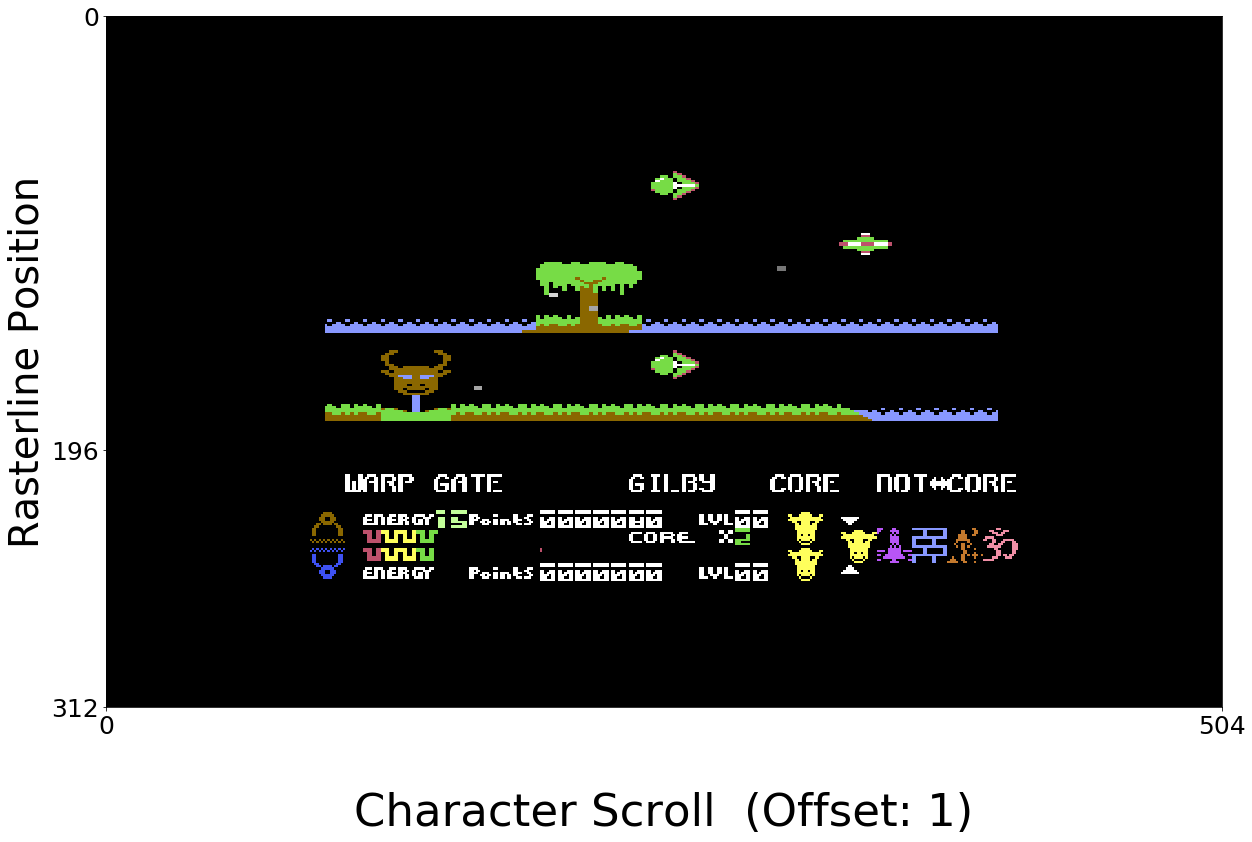
\includegraphics[width=7cm]{main_game/scroll/scroll1770.png}%
\caption{The rasterline positiion at 196 when \icode{ScrollPlanets} is called.}
\end{figure}

Just like with calculating the more fine-grained pixel offset we used \icode{planetScrollSpeed} to determine
how much to move by. But whereas the pixel movement used the lower 3 bits of \icode{planetScrollSpeed} to come
up with a value between 0 and 7 to adjust the pixel scroll by, we will here instead use the 3 bits before that.

The reason for doing that is straightforward: if those upper 3 bits are set the number in \icode{planetScrollSpeed}
must be fairly large and therefore enough to warrant scrolling an entire character or even more.

In a situation where we're moving to the right, this is the logic that figures out how many characters to move and
updates \icode{planetTextureTopLayerPtr} with the updated position:

\begin{lstlisting}
ScrollPlanetRight   
        LDA planetScrollSpeed
        EOR #$FF
        CLC
        AND #$F8
        ROR
        ROR
        ROR
        STA tempHiPtr1
        INC tempHiPtr1
        LDA planetTextureTopLayerPtr
        CLC
        ADC tempHiPtr1
        STA planetTextureTopLayerPtr
\end{lstlisting}

This is more complicated than we actually had reason to expect. Surely if the value in \icode{planetScrollSpeed} is
greater than 7 we could just shift the bits over there and use that instead? For example with a notional value of
\icode{\$1F} in \icode{planetScrollSpeed} if we just did the following:

\begin{lstlisting}
ScrollPlanetRight   
        LDA planetScrollSpeed
        AND #$F8
        ROR
        ROR
        ROR
\end{lstlisting}

We would get a value of \icode{\$03} for our number of characters to move by. THis is because \icode{AND}'ing
\icode{\$1F} and \icode{\$F8} gives us \icode{\$18}:


\begin{figure}[H]
  {
    \setlength{\tabcolsep}{3.0pt}
    \setlength\cmidrulewidth{\heavyrulewidth} % Make cmidrule = 
    \begin{adjustbox}{width=6cm,center}

      \begin{tabular}{rllllllll}
        \toprule
        Byte & Bit 7 & Bit 6 & Bit 5 & Bit 4 & Bit 3 & Bit 2 & Bit 1 & Bit 0        \\
        \midrule
        \$1F & 0 & 0 & 0 & 1 & 1 & 1 & 1 & 1 \\
        \$F8 & 1 & 1 & 1 & 1 & 1 & 0 & 0 & 0 \\
        \midrule
        Result: \$18 & 0 & 0 & 0 & 1 & 1 & 0 & 0 & 0 \\
        \addlinespace
        \bottomrule
      \end{tabular}
    \end{adjustbox}
  }
\end{figure}

And then using \icode{ROR} to shift the bits to the right three times results in \icode{\$03}:

\begin{figure}[H]
  {
    \setlength{\tabcolsep}{3.0pt}
    \setlength\cmidrulewidth{\heavyrulewidth} % Make cmidrule = 
    \begin{adjustbox}{width=6cm,center}

      \begin{tabular}{rllllllll}
        \toprule
        Byte & Bit 7 & Bit 6 & Bit 5 & Bit 4 & Bit 3 & Bit 2 & Bit 1 & Bit 0        \\
        \midrule
        \$18 & 0 & 0 & 0 & 1 & 1 & 0 & 0 & 0 \\
        \midrule
        Result: \$03 & 0 & 0 & 0 & 0 & 0 & 0 & 1 & 1 \\
        \addlinespace
        \bottomrule
      \end{tabular}
    \end{adjustbox}
  }\caption{\icode{ROR} performed three times shifts everything to the right by three bits.}
\end{figure}

But instead of this we're doing an exclusive-or with the value in \icode{planetScrollSpeed} first:

\begin{lstlisting}
ScrollPlanetRight   
        LDA planetScrollSpeed
        EOR #$FF
\end{lstlisting}

The reason we have to do this is because the value in \icode{planetScrollSpeed} isn't what we might have
assumed: a linear value between 0 and 40 for example that goes up and down a sliding scale depending on
how fast we're going. Instead, it's something slightly different. It's fed by the value in \icode{currentGilbySpeed}
that reflects the current velocity of the gilby and this always starts out at a value of \icode{\$EA}:

\begin{lstlisting}
SetUpGilbySprite
        LDA #GILBY_AIRBORNE_RIGHT
        STA currentGilbySprite
        ..
        LDA #$EA
        STA currentGilbySpeed
        ..
        RTS
\end{lstlisting}

There's a trick at work here. The gilby can move left or right and \icode{currentGilbySpeed} is being used to
store both the speed *and* direction of the gilby. When the value is between \icode{00} and \icode{80} the gilby is moving
to the left and the value reflects its relative velociy. When the value is between \icode{80} and \icode{FF} the gilby is
moving to the right and the value reflects its relative velocity.


\begin{figure}[H]
  {
    \setlength{\tabcolsep}{3.0pt}
    \setlength\cmidrulewidth{\heavyrulewidth} % Make cmidrule = 
    \begin{adjustbox}{width=6cm,center}

      \begin{tabular}{rllllllll}
        \toprule
        When Moving Left &  & & & Stationary &  & & & When Moving Right    \\
        \midrule
        \$04 & 03 & 02 & 01 & 00 & FF & FE & FD & FC \\
        \addlinespace
        \bottomrule
      \end{tabular}
    \end{adjustbox}
  }\caption{Value of \icode{currentGilbySpeed} when moving left and right.}
\end{figure}

Sure enough, when we look at the calculation using for the character scroll offset when moving left, it's what we
originally envisaged:

\begin{lstlisting}
ScrollPlanetLeft
        LDA planetScrollSpeed
        CLC
        ADC currentGilbySpeed
        STA planetScrollSpeed
        ..
b72CF   CLC
        ROR
        ROR
        ROR
        STA tempHiPtr1

        LDA planetTextureTopLayerPtr
        SEC
        SBC tempHiPtr1
\end{lstlisting}

So the extra steps we see in \icode{ScrollPlanetRight} are to handle the fact that the speed is going to be some value
between \icode{\$80} and \icode{\$FF}. The exclusive-or (\icode{EOR}) has the effect of reversing the value in \icode{planetScrollSpeed}
and transforming it into a number between 0 and 16 that we can then clamp to a number between 0 and 7.


\begin{lstlisting}
ScrollPlanetRight   
        LDA planetScrollSpeed
        EOR #$FF
        CLC
        AND #$F8
        ROR
        ROR
        ROR
        STA tempHiPtr1
        INC tempHiPtr1
        LDA planetTextureTopLayerPtr
        CLC
        ADC tempHiPtr1
        STA planetTextureTopLayerPtr
\end{lstlisting}


\subsection{Jumping Up and Down}
\begin{lstlisting}[caption=The routines responsible for updating the Gilby's vertical position.]
;-------------------------------------------------------
; PerformMainGameUpdate
;-------------------------------------------------------
PerformMainGameUpdate
        ...
        JSR CalculateGilbyVerticalPositionEarthBound
        JSR CalculateGilbyVerticalPositionAirborne
        ...

\end{lstlisting}
When the gilby jumps on the surface of the planet it exhibits a smooth and pleasing acceleration in ascent and descent that
eloquently suggests the gravity of the planet. This is achieved with a remarkably simple mechanism. Rather than define
distinct behaviours for the journey upwards and the journey back, we use a single continuous movement based on incrementing
the gilby's vertical position with an offset that 'cycles around' and transitions naturally from ascent to descent.

Achieving the complementary movements of ascent and descent with the same operation depends on a simple property of byte values when we increment them. If we keep adding
to a value and it eventually reaches the maximum value of 255 (i.e. \icode{\$FF}) that can be stored in a single byte,
 the next time we add 1 to it it will cycle around to \icode{\$00}. So if we add \icode{\$FB}, for example, to \icode{\$09} 
 we get \icode{\$05}. 

So let's take our starting vertical position (our Y co-ordinate) on the planet to be \icode{\$6D}. This is the Y-coordinate on the
screen that coincides with the surface of the planet. If we're planning to move upwards we might think that the natural number
to subtract from this position to move us up the screen is something like 3 or 4. And then when we're moving down the screen later
on we would increment this position value by 3 or 4, or some smaller number depending on how quickly we want to move. This intuition
is correct, up to a point, but it would mean keeping track of which direction we're going and complicate our code.

Given the circular property of byte arithmetic we described above we can increment or decrement our position by simply adding a carefully
chosen value. If we add a number that will force the result to cycle around and come out less than the current Y value then we've
succesfully subtracted from Y while adding to it! This the essence of our trick.

If we choose our offset value (\icode{gilbyLandingJumpingAnimationYPosOffset}) as \icode{\$FB} and add it to our current Y co-ordinate
of \icode{\$67} we get a result of \icode{\$62}: we move the gilby up the screen by five pixels:

\begin{figure}[H]
    \centering
      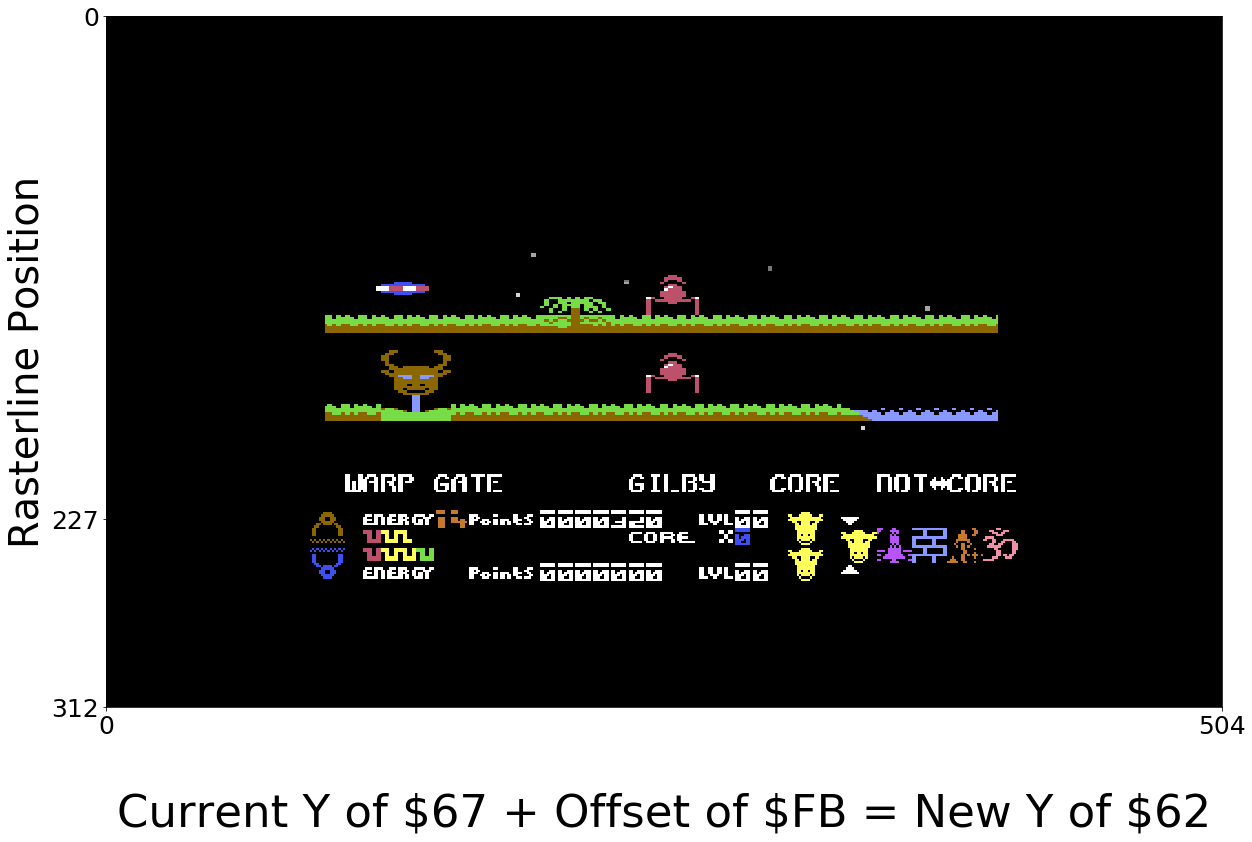
\includegraphics[width=7cm]{main_game/gilby_jumping/gilby_jumping41.png}%
      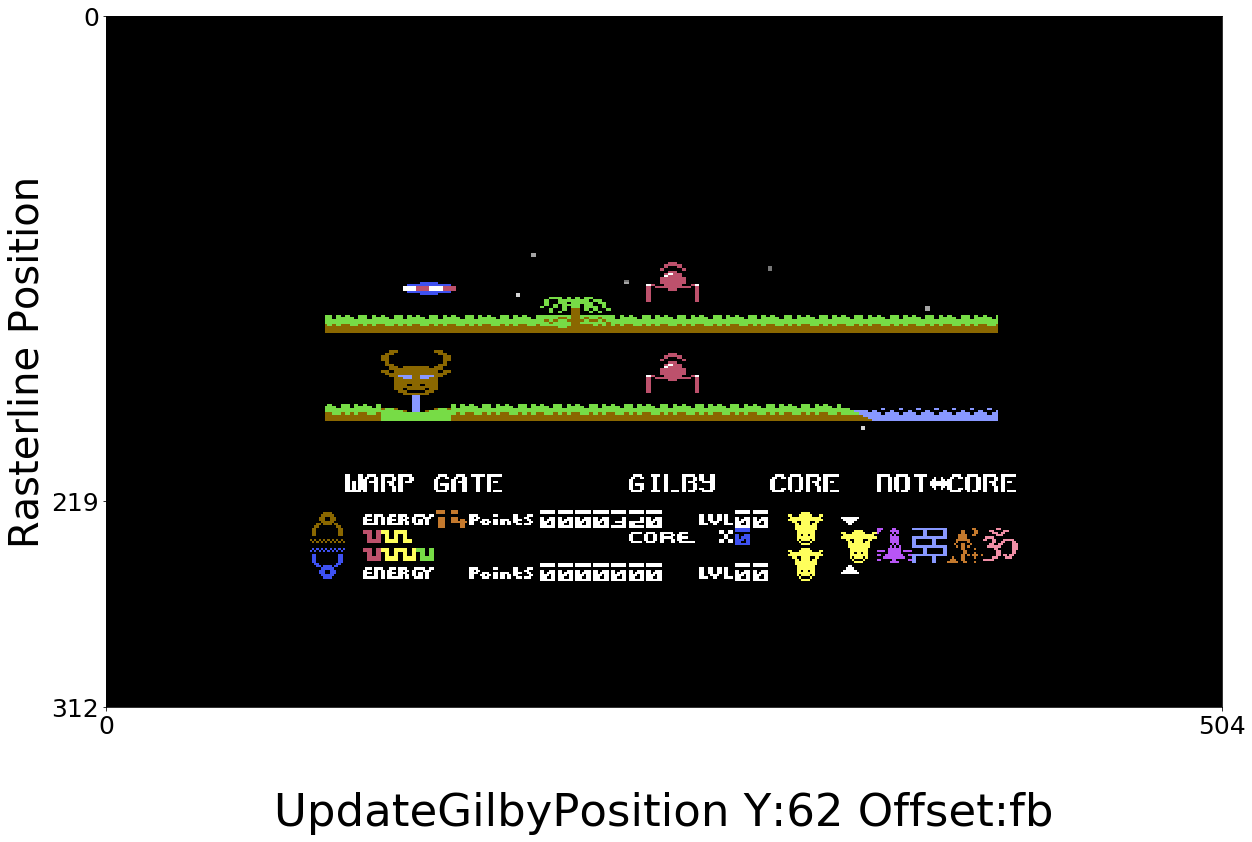
\includegraphics[width=7cm]{main_game/gilby_jumping/gilby_jumping42.png}%
\end{figure}

This is what the code achieving this effect looks like:

\begin{lstlisting}
UpdateGilbyPosition
        CLC
        ADC gilbyLandingJumpingAnimationYPosOffset
        STA gilbyVerticalPositionUpperPlanet

        ; Check if we've hit the surface.
        AND #$F0
        CMP #YPOS_PLANET_SURFACE + $03
        BNE StorePositionAndReturn

        LDA #YPOS_PLANET_SURFACE
        STA gilbyVerticalPositionUpperPlanet

StorePositionAndReturn   
        ; Update the position on screen.
        LDA gilbyVerticalPositionUpperPlanet
        STA $D001    ;Sprite 0 Y Pos
        RTS
\end{lstlisting}

Our choice of \icode{\$FB} as an initial value for the offset is very deliberate. As we increment this offset it will eventually
reach \icode{\$FF}. Each time we do so the resulting degree in movement it creates gets smaller. So the gilby will appear to 
move quickly at first but slow down the further it gets from the planet:

\begin{figure}[H]
    \centering
    \foreach \l in {3,...,11}
    {
      \includegraphics[width=4cm]{main_game/gilby_jumping/gilby_jumping\l.png}%
    }%
\end{figure}

\begin{figure}[H]
    \centering
    \foreach \l in {12,...,17}
    {
      \includegraphics[width=4cm]{main_game/gilby_jumping/gilby_jumping\l.png}%
    }%
\caption{Each increment in the offset, performed every three movements, results in a deceleration effect.}
\end{figure}

When our offset value \icode{gilbyLandingJumpingAnimationYPosOffset} reaches \icode{\$FF} it is time for modular arithmetic
to kick in the next time we increment it: the movement-increment it gives us is \icode{\$00} and for the next three 'movements' the gilby appears to
hang in the sky at Y co-ordinate \icode{\$33}:

\begin{figure}[H]
    \centering
    \foreach \l in {18,...,20}
    {
      \includegraphics[width=4cm]{main_game/gilby_jumping/gilby_jumping\l.png}%
    }%
\end{figure}

Now that \icode{gilbyLandingJumpingAnimationYPosOffset} is \icode{\$00} adding it to our current Y position will no longer have the 
effect of cycling around and arriving a smaller value than the current Y position. Instead it will increment the Y position and move
the gilby down the screen again. Just as when we were moving upwards the resulting movement increases in degree as we get closer to the
land, creating an acceleration effect due to gravity. 

\begin{figure}[H]
    \centering
    \foreach \l in {21,...,35}
    {
      \includegraphics[width=4cm]{main_game/gilby_jumping/gilby_jumping\l.png}%
    }%
\caption{Each increment in the offset, performed every three movements, results in an acceleration effect.}
\end{figure}

With a simple, consistent addition operation each time it comes to position the gilby we've managed to achieve a jumping and
landing effect with a neat gravity effect built in!

\subsection{Sound Effects}
\begin{lstlisting}
;-------------------------------------------------------
; PerformMainGameUpdate
;-------------------------------------------------------
PerformMainGameUpdate
        ...
        JSR PlaySoundEffects
        ...
\end{lstlisting}

Iridis Alpha has a rich weave of sound effects during play. The game is as much an assault on the ears as it is on
the eyes. In order to create the impression that there are multiple sounds going on at once so it is necessary to... have
multiple sounds going at once. The fancy word for this is 'multiplexing'. If we want the player to experience the world
of Iridis Alpha as one in which things are not happening sequentially but simultaneously we will need the sounds they
experience to interleave with each other, rather than just playing whatever the 'current' sound is then waiting for it
to finish before we play the next. Playing two sounds at once is more than enough multiplexing to be going on with,
so that is what we do. 

The way to achieve this is to come up with a data structure for sound effects that segments the full sound effect
into multiple frames and to process a few frames of each data structure every time \icode{PlaySoundEffects} is called
by the raster interrupt. We also need \icode{PlaySoundEffects} to behave like a 'state machine'. This means that
when it is called a little later it can pick up from where it left off on each data structure, recognize
when it has finished playing the frames for that interrupt and also when it has finished playing the full effect. This
will allow us to manage two different sound effects concurrently. Before we look at how this multiplexing is achieved
lets look at how a single sound effect is managed in general.

\subsubsection{The Sound Effect Data Structure}
As ever, the key to managing complexity isn't the cleverness of our code but the simplicity of the data structure
we choose. Iridis Alpha solves this with a remarkably compact solution where each frame in the sound effect is represented
by a meagre 5 bytes and the whole sound effect is encoded by a sequence of these 5-byte records. In order to unpack
what this looks like in practice, let's look at the iconic effect played when we enter a new planet. The data structure
here is just one part of the level entry sound effect, the duller part. It plays a dull bass note that fades away. (We'll
examine the more interesting leg of the overall sound effect, the one that it's multiplexed with, right after this. But
this is a relatively nice and simple one for us to get an idea of how the data structure works.) 

\begin{lstlisting}
PLAY_SOUND = $00
PLAY_LOOP = $05
LINK = $80
VOICE2_HI = $08
VOICE2_CTRL = $0B
VOICE3_HI = $0F
VOICE2_ATK_DEC = $0C
VOICE2_SUS_REL = $0D
VOICE3_CTRL = $12
VOICE3_ATK_DEC = $13
VOICE3_SUS_REL = $14
planetWarpSoundEffect  .BYTE $00,PLAY_SOUND,$0F,VOICE2_ATK_DEC,$00
                       .BYTE $00,PLAY_SOUND,$0F,VOICE3_ATK_DEC,$00
                       .BYTE $00,PLAY_SOUND,$0F,VOLUME,$00
                       .BYTE $00,PLAY_SOUND,$00,VOICE2_SUS_REL,$00
                       .BYTE $00,PLAY_SOUND,$00,VOICE3_SUS_REL,$00
                       .BYTE $00,PLAY_SOUND,$03,VOICE2_HI,$00
                       .BYTE $00,PLAY_SOUND,$03,VOICE3_HI,$00
                       .BYTE $00,PLAY_SOUND,$21,VOICE2_CTRL,$00
                       .BYTE $00,PLAY_SOUND,$08,VOICE3_LO,$00
                       .BYTE $00,PLAY_SOUND,$00,VOICE2_LO,$00
pwLoop                 .BYTE $00,PLAY_SOUND,$21,VOICE3_CTRL,$01
                       .BYTE $18,PLAY_LOOP,$00,<pwLoop,>pwLoop
                       .BYTE $00,PLAY_SOUND,$20,VOICE2_CTRL,$00
                       .BYTE $00,PLAY_SOUND,$20,VOICE3_CTRL,$00
                       .BYTE $00,LINK,<setVolToMax,>setVolToMax,$00
\end{lstlisting}

This data is like a piano roll fed into \icode{PlaySoundEffects}. In simplified terms each line is a 'frame' containing
a single note for it to play. For the lines with \icode{PLAY\_SOUND} it really is that simple. Byte 3 in each of those lines
is the 'note' to play, and Byte 4 (e.g. \icode{VOICE2\_ATK\_DEC} is the 'key on the piano' to play it on. \icode{PlaySoundEffects}
will keep playing each line in the roll until it hits one with a value in Byte 5 that is not \icode{\$00}. In this case that
happens when it hits the line that starts with \icode{pwLoop}, notice the \icode{\$01} at the very end.

Let's be more concrete about what's happening when each \icode{PLAY\_SOUND} record is processed as it's quite simple. The value in Byte 3 
is written to the position in the SID register given by Byte 4. The SID register is an array of bytes in the C64's ROM that controls
the production of sound and they live between addresses \icode{\$D400} and \icode{\$D418}. So in the first record in \icode{planetWarpSoundEffect}
we are going to write \icode{\$0F} to the address \icode{\$D40C} in the SID register. 

What does that do you might ask? Does it play a note? Well, no, as it happens this address in the SID register is responsible for
controlling how much a sound rises or falls. As you can see in the visualization of the effect below it decays away. This byte
we're setting is reponsible for setting that on 'Voice 2' in the sound chip.  

\begin{figure}[H]
{
\setlength{\tabcolsep}{1.0pt}
\setlength\cmidrulewidth{\heavyrulewidth} % Make cmidrule = 
\begin{adjustbox}{width=14cm,center}
\begin{tabular}{ccc}
\toprule
Spectrogram & Amplitude & Sound \\
\midrule
  \makecell[l]{
    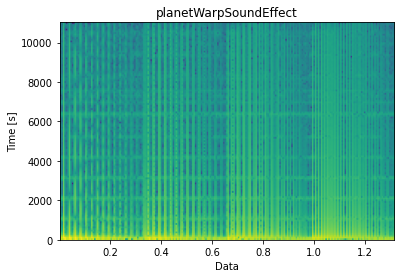
\includegraphics[width=6cm]{sound_effects/planetWarpSoundEffect.wav-spec.png}%
  } &
  \makecell[l]{
    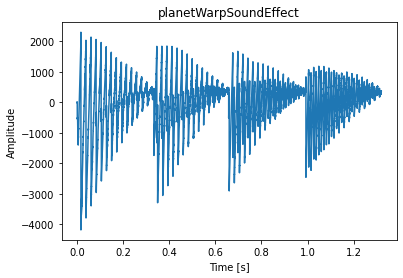
\includegraphics[width=6cm]{sound_effects/planetWarpSoundEffect.wav-amp.png}%
  } &
  \makecell[l]{
    \textattachfile{src/sound_effects/sounds/planetWarpSoundEffect.wav}{
\includegraphics[width=1cm]{sound_effects/sounds/play.png}}
  } \\
  \addlinespace
    \bottomrule
    \end{tabular}
  \end{adjustbox}
}\caption{}
\end{figure}

The next record does the same for 'Voice 3'. The one after that sets the volume (\icode{\$D418}) to its maximum value of 15 (\icode{\$0F}.
\begin{lstlisting}
               .BYTE $00,PLAY_SOUND,$0F,VOICE3_ATK_DEC,$00
               .BYTE $00,PLAY_SOUND,$0F,VOLUME,$00
\end{lstlisting}

The next two records ensure Voices 2 and 3 do not sustain their sound by writing \icode{\$00} to both. We just want them to die
away quickly after all.
\begin{lstlisting}
               .BYTE $00,PLAY_SOUND,$00,VOICE2_SUS_REL,$00
               .BYTE $00,PLAY_SOUND,$00,VOICE3_SUS_REL,$00
\end{lstlisting}

Finally we can start playing some notes.
\begin{lstlisting}
               .BYTE $00,PLAY_SOUND,$03,VOICE2_HI,$00
               .BYTE $00,PLAY_SOUND,$03,VOICE3_HI,$00
\end{lstlisting}

What we are doing here is writing a frequency value to SID registers for Voice 2 and Voice 3 that will actually make some noise.
We then tell the sound device to start playing the note by setting its 'gate' to 1. The 'gate' is the 'least significant bit', i.e.
the \icode{1} in the \icode{\$21} given in Byte 3:

\begin{lstlisting}
               .BYTE $00,PLAY_SOUND,$21,VOICE2_CTRL,$00
\end{lstlisting}

After adjusting the sound again:


\begin{lstlisting}
               .BYTE $00,PLAY_SOUND,$08,VOICE3_LO,$00
               .BYTE $00,PLAY_SOUND,$00,VOICE2_LO,$00
\end{lstlisting}

We now encounter the use of a new record type called \icode{PLAY\_LOOP}. 

\begin{lstlisting}
VOLUME = $18
pwLoop        .BYTE $00,PLAY_SOUND,$21,VOICE3_CTRL,$01
              .BYTE VOLUME,PLAY_LOOP,$01,<pwLoop,>pwLoop
\end{lstlisting}

What this this particular instance of a \icode{PLAY\_LOOP} record does is gradually lower the volume until it reaches zero.

More generally the way \icode{PLAY\_LOOP} records are processed is as follows. First of all we write to the offset in the SID register 
given by Byte 1 (in this case the register responsible for volume). The value we write is also derived from Byte 1, but by using it
as in index into an array called \icode{soundEffectBuffer}:

\begin{lstlisting}
soundEffectBuffer   .BYTE $00,$94,$00,$00,$11,$0F,$00,$00
                    .BYTE $03,$00,$00,$21,$0F,$00,$08,$03
                    .BYTE $00,$00,$21,$0F,$00,$00,$00,$00
                    .BYTE $02,$00,$00,$00,$00,$00,$00,$00
\end{lstlisting}


If we look at our record again..

\begin{lstlisting}
              .BYTE VOLUME,PLAY_LOOP,$01,<pwLoop,>pwLoop
\end{lstlisting}

we can see Byte 1 is \icode{VOLUME}, which is an alias for the value \icode{\$18}. Using \icode{\$18} as an index into
\icode{soundEffectBuffer} retrieves the fourth value on the third line above, \icode{\$0F}. We then subtract the value
in Byte 3 (\icode{\$01}) and store the result back in the \icode{soundEffectBuffer}. If it's not zero yet,
we then treat the record pointed to by Bytes 4 and 5 as the next one to play. In this case thats given as \icode{pwLoop}. So in
fact we go round in a loop between the two records until \icode{\$0F} eventually becomes zero. Here's the code that handles this:


\begin{lstlisting}
        LDX soundEffectDataStructure_Byte1
        LDA soundEffectBuffer,X
        SEC
        SBC soundEffectDataStructure_Byte3

StorePointersAndReturnIfZero
        STA soundEffectBuffer,X
        STA $D400,X  ;Voice 1: Frequency Control - Low-Byte
        BEQ JumpToGetNextRecordInSoundEffect
        LDA soundEffectDataStructure_Byte4
        LDX indexToPrimaryOrSecondarySoundEffectPtr
        STA primarySoundEffectLoPtr,X
        LDA soundEffectDataStructure_Byte5
        STA primarySoundEffectHiPtr,X
        RTS

JumpToGetNextRecordInSoundEffect   
        JMP GetNextRecordInSoundEffect
\end{lstlisting}

You can see that once we reach zero \icode{BEQ JumpToGetNextRecordInSoundEffect} becomes true and we end up calling 
\icode{GetNextRecordInSoundEffect} which actually lets us move on to the next record in our data structure (the two
we've just looped through are given at the start to make it easier to see where picked up from):

\begin{lstlisting}
               .BYTE $00,PLAY_SOUND,$20,VOICE2_CTRL,$00
               .BYTE $00,PLAY_SOUND,$20,VOICE3_CTRL,$00
\end{lstlisting}

You can see we write \icode{\$20} to \icode{VOICE2\_CTRL} and \icode{VOICE3\_CTRL}. This stops the noise we were making
until now. It switches off the sound by setting the 'gate' we set to \icode{1} earlier on back to \icode{0}.

The final record we play is a simple 'jump' record. Its processed by simply jumping to the address given in Bytes 4 and
5 and playing whatever is there:

\begin{lstlisting}
              .BYTE $00,LINK,<setVolToMax,>setVolToMax,$00
\end{lstlisting}

In this case it is pointing us to the data structure at \icode{setVolToMax}. This simply runs in a loop setting the volume
back to \icode{\$0F}, i.e. it's maximum value of 15. Notice the way the firs record below writes \icode{\$0F} (Byte 3) to the
\icode{VOLUME} register. The second one, just tells it loop back and do the same thing again. This will keep running until
a new sound effect is selected.

\begin{lstlisting}
setVolToMax            .BYTE $00,PLAY_SOUND,$0F,VOLUME,$01
                       .BYTE $00,LINK,<setVolToMax,>setVolToMax,$00
\end{lstlisting}

We can get a picture of how each record affects the relevant registers in the SID interface by looking at the table below.
This is full history of each record that's processed in the \icode{planetWarpSoundEffect} data structure by \icode{PlaySoundEffects}
in temporal order. Notice the way the colume steadily decreases as we go through the \icode{PLAY\_LOOP} loop towards the end.

\begin{figure}[H]
{
  \setlength{\tabcolsep}{3.0pt}
  \setlength\cmidrulewidth{\heavyrulewidth} % Make cmidrule = 
    \begin{adjustbox}{width=\textwidth}

  \begin{tabular}{lrrrrrrrrr}
  \hline
    Data Frame &   Voice 2 &   &   &   &   Voice 3 &   &   &   & Volume \\
    &   Sound &   Gate &   Saw &   Decay &   Sound &   Gate &   Saw &   Decay &    \\
    \hline
    \icode{\$00,PLAY\_SOUND,\$0F,VOICE3\_ATK\_DEC,\$00} &       0 &       0 &      0 &     15 &       0 &       0 &      0 &      0 &    15 \\
    \icode{\$00,PLAY\_SOUND,\$0F,VOLUME,\$00}         &       0 &       0 &      0 &     15 &       0 &       0 &      0 &     15 &    15 \\
    \icode{\$00,PLAY\_SOUND,\$00,VOICE2\_SUS\_REL,\$00} &       0 &       0 &      0 &     15 &       0 &       0 &      0 &     15 &    15 \\
    \icode{\$00,PLAY\_SOUND,\$00,VOICE3\_SUS\_REL,\$00} &       0 &       0 &      0 &     15 &       0 &       0 &      0 &     15 &    15 \\
    \icode{\$00,PLAY\_SOUND,\$03,VOICE2\_HI,\$00}      &     768 &       0 &      0 &     15 &       0 &       0 &      0 &     15 &    15 \\
    \icode{\$00,PLAY\_SOUND,\$03,VOICE3\_HI,\$00}      &     768 &       0 &      0 &     15 &     768 &       0 &      0 &     15 &    15 \\
    \icode{\$00,PLAY\_SOUND,\$21,VOICE2\_CTRL,\$00}    &     768 &       1 &      1 &     15 &     768 &       0 &      0 &     15 &    15 \\
    \icode{\$00,PLAY\_SOUND,\$08,VOICE3\_LO,\$00}      &     768 &       1 &      1 &     15 &     776 &       0 &      0 &     15 &    15 \\
    \icode{\$00,PLAY\_SOUND,\$00,VOICE2\_LO,\$00}      &     768 &       1 &      1 &     15 &     776 &       0 &      0 &     15 &    15 \\
    \icode{\$00,PLAY\_SOUND,\$21,VOICE3\_CTRL,\$01}    &     768 &       1 &      1 &     15 &     776 &       1 &      1 &     15 &    15 \\
    \icode{\$18,PLAY\_LOOP,\$00,\ensuremath{<}pwLoop,\ensuremath{>}pwLoop}       &     768 &       1 &      1 &     15 &     776 &       1 &      1 &     15 &    14 \\
    \icode{\$00,PLAY\_SOUND,\$21,VOICE3\_CTRL,\$01}    &     768 &       1 &      1 &     15 &     776 &       1 &      1 &     15 &    13 \\
    \icode{\$18,PLAY\_LOOP,\$00,\ensuremath{<}pwLoop,\ensuremath{>}pwLoop}       &     768 &       1 &      1 &     15 &     776 &       1 &      1 &     15 &    12 \\
    \icode{\$00,PLAY\_SOUND,\$21,VOICE3\_CTRL,\$01}    &     768 &       1 &      1 &     15 &     776 &       1 &      1 &     15 &    11 \\
    \icode{\$18,PLAY\_LOOP,\$00,\ensuremath{<}pwLoop,\ensuremath{>}pwLoop}       &     768 &       1 &      1 &     15 &     776 &       1 &      1 &     15 &    10 \\
    \icode{\$00,PLAY\_SOUND,\$21,VOICE3\_CTRL,\$01}    &     768 &       1 &      1 &     15 &     776 &       1 &      1 &     15 &     9 \\
    \icode{\$18,PLAY\_LOOP,\$00,\ensuremath{<}pwLoop,\ensuremath{>}pwLoop}       &     768 &       1 &      1 &     15 &     776 &       1 &      1 &     15 &     8 \\
    \icode{\$00,PLAY\_SOUND,\$21,VOICE3\_CTRL,\$01}    &     768 &       1 &      1 &     15 &     776 &       1 &      1 &     15 &     7 \\
    \icode{\$18,PLAY\_LOOP,\$00,\ensuremath{<}pwLoop,\ensuremath{>}pwLoop}       &     768 &       1 &      1 &     15 &     776 &       1 &      1 &     15 &     6 \\
    \icode{\$00,PLAY\_SOUND,\$21,VOICE3\_CTRL,\$01}    &     768 &       1 &      1 &     15 &     776 &       1 &      1 &     15 &     5 \\
    \icode{\$18,PLAY\_LOOP,\$00,\ensuremath{<}pwLoop,\ensuremath{>}pwLoop}       &     768 &       1 &      1 &     15 &     776 &       1 &      1 &     15 &     4 \\
    \icode{\$00,PLAY\_SOUND,\$21,VOICE3\_CTRL,\$01}    &     768 &       1 &      1 &     15 &     776 &       1 &      1 &     15 &     3 \\
    \icode{\$18,PLAY\_LOOP,\$00,\ensuremath{<}pwLoop,\ensuremath{>}pwLoop}       &     768 &       1 &      1 &     15 &     776 &       1 &      1 &     15 &     2 \\
    \icode{\$00,PLAY\_SOUND,\$21,VOICE3\_CTRL,\$01}    &     768 &       1 &      1 &     15 &     776 &       1 &      1 &     15 &     1 \\
    \icode{\$18,PLAY\_LOOP,\$00,\ensuremath{<}pwLoop,\ensuremath{>}pwLoop}       &     768 &       1 &      1 &     15 &     776 &       1 &      1 &     15 &     0 \\
    \icode{\$00,PLAY\_SOUND,\$21,VOICE3\_CTRL,\$01}    &     768 &       0 &      1 &     15 &     776 &       1 &      1 &     15 &     0 \\
    \icode{\$18,PLAY\_LOOP,\$00,\ensuremath{<}pwLoop,\ensuremath{>}pwLoop}       &     768 &       0 &      1 &     15 &     776 &       0 &      1 &     15 &     0 \\
  \hline
    \end{tabular}

  \end{adjustbox}

}\caption*{}
\end{figure}

\subsubsection{Multiplexing}
While playing the fairly dull component we cover above, Iridis Alpha plays a second sequence simultaneously that constitutes
the one a player will know and recognize.

\begin{figure}[H]
{
\setlength{\tabcolsep}{1.0pt}
\setlength\cmidrulewidth{\heavyrulewidth} % Make cmidrule = 
\begin{adjustbox}{width=14cm,center}
\begin{tabular}{ccc}
\toprule
Spectrogram & Amplitude & Sound \\
\midrule
    \makecell[l]{
      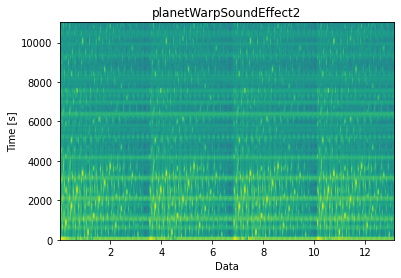
\includegraphics[width=6cm]{sound_effects/planetWarpSoundEffect2.wav-spec.png}%
    } &
  \makecell[l]{
    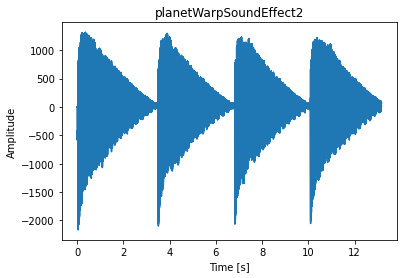
\includegraphics[width=6cm]{sound_effects/planetWarpSoundEffect2.wav-amp.png}%
  } &
  \makecell[l]{
    \textattachfile{src/sound_effects/sounds/planetWarpSoundEffect2.wav}{
\includegraphics[width=1cm]{sound_effects/sounds/play.png}}
  } \\
  \addlinespace
    \bottomrule
    \end{tabular}
  \end{adjustbox}
}\caption{}
\end{figure}

The way this concurrency is managed is by storing the addresses for each effect separately. In the case of the sequence
where the player is entering a new planet this is done in \icode{PerformPlanetWarp}, the routine responsible for rendering
the warp sequence as a whole:

\begin{lstlisting}
PerformPlanetWarp
        ...
        LDA #<planetWarpSoundEffect
        STA secondarySoundEffectLoPtr
        LDA #>planetWarpSoundEffect
        STA secondarySoundEffectHiPtr
        LDA #<planetWarpSoundEffect2
        STA primarySoundEffectLoPtr
        LDA #>planetWarpSoundEffect2
        STA primarySoundEffectHiPtr
\end{lstlisting}

With the primary and secondary sound effects stored in \icode{primarySoundEffectLo/HIPtr} and \icode{secondarySoundEffectLo/HiPtr}
respectively, all the \icode{PlaySoundEffects} routine has to do it ensures that it processes each of the effects every time it
is visited by the raster interrupt.  Here we see it take in the 'primary' sound effect and process it in \icode{PlayCurrentSoundEffect}:

\begin{lstlisting}
PlaySoundEffects
        LDA #$00
        STA indexToPrimaryOrSecondarySoundEffectPtr
        LDA soundEffectInProgress
        BEQ DontDecrementSoundEffectProgressCounter
        DEC soundEffectInProgress
DontDecrementSoundEffectProgressCounter   
        LDA primarySoundEffectLoPtr
        STA currentSoundEffectLoPtr
        LDA primarySoundEffectHiPtr
        STA currentSoundEffectHiPtr
        JSR PlayCurrentSoundEffect
\end{lstlisting}

And here we see it then move on to processing the \icode{secondarySoundEffect}. Notice that it falls through to \icode{PlayCurrentSoundEffect}
rather than having to call it directly with \icode{JSR}:

\begin{lstlisting}
        LDA #$02
        STA indexToPrimaryOrSecondarySoundEffectPtr
        LDA secondarySoundEffectLoPtr
        STA currentSoundEffectLoPtr
        LDA secondarySoundEffectHiPtr
        STA currentSoundEffectHiPtr
        ;Falls through and plays secondary sound effect.

;-------------------------------------------------------
; PlayCurrentSoundEffect
;-------------------------------------------------------
PlayCurrentSoundEffect
        LDY #$00
        ; Read the 5-byte record into working storage.
FillSoundEffectDataStructureLoop   
        LDA (currentSoundEffectLoPtr),Y
        STA soundEffectDataStructure,Y
        INY
        CPY #$05
        BNE FillSoundEffectDataStructureLoop

\end{lstlisting}

The secondary sound effect for the planet warp sequence, which is the one with all the recognizable noises, looks like this:

\begin{lstlisting}
          .BYTE $00,PLAY_SOUND,$0F,VOICE1_ATK_DEC,$00
          .BYTE $00,PLAY_SOUND,$00,VOICE1_SUS_REL,$00
          .BYTE $00,PLAY_SOUND,$00,VOICE1_HI,$00
pwLoop    .BYTE $00,PLAY_SOUND,$11,VOICE1_CTRL,$02
          .BYTE $01,INC_AND_PLAY_FROM_BUFFER,$64,VOICE1_HI,$01
          .BYTE $00,REPEAT_PREVIOUS,$08,$00,$00
          .BYTE $01,INC_AND_PLAY_FROM_BUFFER,$18,VOICE1_HI,$01
          .BYTE VOLUME,PLAY_LOOP,$01,<pwLoop,>pwLoop
          .BYTE $00,PLAY_SOUND,$10,VOICE1_CTRL,$00
          .BYTE $00,LINK,<setVolumeToMax,>setVolumeToMax,$00
\end{lstlisting}

Just like the primary sound effect we discussed this one contains a loop, achieving the same effect as before. 
There are a couple of new record types in there though, namely \icode{INC\_AND\_PLAY\_FROM\_BUFFER} and \icode{REPEAT\_PREVIOUS}.
The latter is probably self-explanatory, it repeats processing of the previous record for as many times as given by the 
value in Byte 3 which in this is case is \icode{\$08} times.

\icode{INC\_AND\_PLAY\_FROM\_BUFFER} does something more interesting, in the first case above it's being used to update the sound we play
(i.e. write to register \icode{VOICE1\_HI}) by a regularly incrementing amounts of \icode{\$64} given in Byte 3. This value is picked
from and updated in position 1 of the \icode{soundEffectBuffer}, this position being given by Byte 1. The result is the 'iconic'
bleeping sound that increases in frequency as we warp into the planet. Here we see the section in \icode{PlaySoundEffects} that
processes records of type \icode{INC\_AND\_PLAY\_FROM\_BUFFER}, and the way it uses each byte in the record to effect the update
and the write to the sound register:

\begin{lstlisting}
        ; Increment the value in the buffer and play it.
        LDX soundEffectDataStructure_Byte1
        LDA soundEffectBuffer,X
        CLC
        ADC soundEffectDataStructure_Byte3
        LDX soundEffectDataStructure_Byte4
        STA soundEffectBuffer,X
        STA $D400,X  ;Voice 1: Frequency Control - Low-Byte
        JMP GetNextRecordAndMaybePlayIt
\end{lstlisting}


\begin{sidewaysfigure}
{
  \setlength{\tabcolsep}{1.0pt}
  \setlength\cmidrulewidth{\heavyrulewidth} % Make cmidrule = 
    \begin{adjustbox}{width=18cm,center}
  \begin{tabular}{llllll}
  \toprule
    Record Type & Byte 1 & Byte 2 & Byte 3 & Byte 4 & Byte 5 \\
    \midrule
    \makecell[l]{
      Play Sound
    } &
    \makecell[l]{
      Unused
    } &
    \makecell[l]{
      PLAY\_SOUND \\
      (\icode{\$00})
    } &
    \makecell[l]{
      Value to write to \\
      offset to \icode{\$D400} \\
      given by Byte 4.
    } &
    \makecell[l]{
      Offset to \icode{\$D400} \\
      to write to.
    } &
    \makecell[l]{
 '00' indicates the next record should be \\
 played immediately. \\
 '01' indicates should play no more records. \\
 Anything else indicates the next record \\
  should be stored and \\
  no more should be played for now. \\
    } \\
    \addlinespace
    \makecell[l]{
Increment and \\
Play from Buffer      
    } &
    \makecell[l]{
      Address of byte \\
      to pick from \\
      \icode{soundEffectBuffer}
    } &
    \makecell[l]{
      INC\_AND\_PLAY\_ \\
      FROM\_BUFFER \\
      (\icode{\$01})
    } &
    \makecell[l]{
      Amount to \\
      increment \\
      picked byte by.
    } &
    \makecell[l]{
      Offset to \icode{\$D400} \\
      to write to.
    } &
    \makecell[l]{
'00' indicates the next record should be \\
played immediately. \\
'01' indicates should play no more records. \\
Anything else indicates the next record \\
should be stored and \\
 no more should be played for now.
    } \\
    \addlinespace
    \makecell[l]{
Decrement and \\
Play from Buffer      
    } &
    \makecell[l]{
      Address of byte \\
      to pick from \\
      \icode{soundEffectBuffer}
    } &
    \makecell[l]{
      DEC\_AND\_PLAY\_ \\
      FROM\_BUFFER \\
      (\icode{\$02})
    } &
    \makecell[l]{
      Amount to \\
      decrement \\
      picked byte by.
    } &
    \makecell[l]{
      Offset to \icode{\$D400} \\
      to write to.
    } &
    \makecell[l]{
'00' indicates the next record should be \\
played immediately. \\
'01' indicates should play no more records. \\
Anything else indicates the next record \\
should be stored and \\
 no more should be played for now.
    } \\
    \addlinespace
    \makecell[l]{
Play Loop\\
    } &
    \makecell[l]{
      Address of byte \\
      to pick from \\
      \icode{soundEffectBuffer} \\
      and offset to \icode{\$D400}
    } &
    \makecell[l]{
      PLAY\_LOOP \\
      (\icode{\$05})
    } &
    \makecell[l]{
      Amount to \\
      decrement \\
      picked byte by.
    } &
    \makecell[l]{
      Lo Ptr of \\
      next record.
    } &
    \makecell[l]{
      Hi Ptr of \\
      next record.
    } \\
    \addlinespace
    \makecell[l]{
Link to\\
Record
    } &
    \makecell[l]{
      Unused.\\
    } &
    \makecell[l]{
      LINK \\
      (\icode{\$80})
    } &
    \makecell[l]{
      Lo Ptr of \\
      next record.
    } &
    \makecell[l]{
      Hi Ptr of \\
      next record.
    } &
    \makecell[l]{
'00' indicates the next record should be \\
played immediately. \\
'01' indicates should play no more records. \\
Anything else indicates the next record \\
should be stored and \\
 no more should be played for now.
    } \\
    \addlinespace
    \makecell[l]{
Repeat \\
Previous \\
Record
    } &
    \makecell[l]{
      Unused.\\
    } &
    \makecell[l]{
      REPEAT\_ \\
      PREVIOUS\\
      (\icode{\$81})
    } &
    \makecell[l]{
      Number of \\
      times to play 
      previous record\.\
    } &
    \makecell[l]{
      Unused.
    } &
    \makecell[l]{
'00' indicates the next record should be \\
played immediately. \\
'01' indicates should play no more records. \\
Anything else indicates the next record \\
should be stored and \\
 no more should be played for now.
    } \\
    \addlinespace
      \bottomrule
      \end{tabular}
  \end{adjustbox}
}\caption{The data structures for sound effects used by Iridis Alpha.}
\end{sidewaysfigure}

The amount of looping the data structure demands is much greater than the effect we reviewed previously. We can get a sense
of this from the truncated trace which shows a total of over 250 writes to the sound register and of which the table below
is just a snapshot:

\begin{figure}[H]
{
  \setlength{\tabcolsep}{3.0pt}
  \setlength\cmidrulewidth{\heavyrulewidth} % Make cmidrule = 
    \begin{adjustbox}{width=\textwidth}

  \begin{tabular}{lrrrrrr}
  \hline
    &   freq1 &   gate1 &   saw1 &   dec1 &   sus1 &   vol \\
    \hline
    \icode{\$00,PLAY\_SOUND,\$0F,VOICE1\_ATK\_DEC,\$00}          &       0 &       0 &      0 &     15 &      0 &    15 \\
    \icode{\$00,PLAY\_SOUND,\$00,VOICE1\_SUS\_REL,\$00}          &       0 &       0 &      0 &     15 &      0 &    15 \\
    \icode{\$00,PLAY\_SOUND,\$00,VOICE1\_HI,\$00}               &       0 &       0 &      0 &     15 &      0 &    15 \\
    \icode{\$00,PLAY\_SOUND,\$11,VOICE1\_CTRL,\$02}             &       0 &       1 &      0 &     15 &      0 &    15 \\
    \icode{\$01,INC\_AND\_PLAY\_FROM\_BUFFER,\$64,VOICE1\_HI,\$01} &   25600 &       1 &      0 &     15 &      0 &    15 \\
    \icode{\$01,INC\_AND\_PLAY\_FROM\_BUFFER,\$64,VOICE1\_HI,\$01} &   51200 &       1 &      0 &     15 &      0 &    15 \\
    \icode{\$01,INC\_AND\_PLAY\_FROM\_BUFFER,\$64,VOICE1\_HI,\$01} &   11264 &       1 &      0 &     15 &      0 &    15 \\
    \icode{\$01,INC\_AND\_PLAY\_FROM\_BUFFER,\$64,VOICE1\_HI,\$01} &   36864 &       1 &      0 &     15 &      0 &    15 \\
    \icode{\$01,INC\_AND\_PLAY\_FROM\_BUFFER,\$64,VOICE1\_HI,\$01} &   62464 &       1 &      0 &     15 &      0 &    15 \\
    \icode{\$01,INC\_AND\_PLAY\_FROM\_BUFFER,\$64,VOICE1\_HI,\$01} &   22528 &       1 &      0 &     15 &      0 &    15 \\
    \icode{\$01,INC\_AND\_PLAY\_FROM\_BUFFER,\$64,VOICE1\_HI,\$01} &   48128 &       1 &      0 &     15 &      0 &    15 \\
    \icode{\$01,INC\_AND\_PLAY\_FROM\_BUFFER,\$64,VOICE1\_HI,\$01} &    8192 &       1 &      0 &     15 &      0 &    15 \\
    \icode{\$01,INC\_AND\_PLAY\_FROM\_BUFFER,\$18,VOICE1\_HI,\$01} &   14336 &       1 &      0 &     15 &      0 &    15 \\
    \icode{VOLUME,PLAY\_LOOP,\$01,\ensuremath{<}f5D8D,\ensuremath{>}f5D8D}             &   14336 &       1 &      0 &     15 &      0 &    14 \\
    \icode{\$00,PLAY\_SOUND,\$11,VOICE1\_CTRL,\$02}             &   39936 &       1 &      0 &     15 &      0 &    14 \\
    \icode{\$01,INC\_AND\_PLAY\_FROM\_BUFFER,\$64,VOICE1\_HI,\$01} &       0 &       1 &      0 &     15 &      0 &    14 \\
    \icode{\$01,INC\_AND\_PLAY\_FROM\_BUFFER,\$64,VOICE1\_HI,\$01} &   25600 &       1 &      0 &     15 &      0 &    14 \\
    \icode{\$01,INC\_AND\_PLAY\_FROM\_BUFFER,\$64,VOICE1\_HI,\$01} &   51200 &       1 &      0 &     15 &      0 &    14 \\
    \icode{\$01,INC\_AND\_PLAY\_FROM\_BUFFER,\$64,VOICE1\_HI,\$01} &   11264 &       1 &      0 &     15 &      0 &    14 \\
    \icode{\$01,INC\_AND\_PLAY\_FROM\_BUFFER,\$64,VOICE1\_HI,\$01} &   36864 &       1 &      0 &     15 &      0 &    14 \\
    \icode{\$01,INC\_AND\_PLAY\_FROM\_BUFFER,\$64,VOICE1\_HI,\$01} &   62464 &       1 &      0 &     15 &      0 &    14 \\
    \icode{\$01,INC\_AND\_PLAY\_FROM\_BUFFER,\$64,VOICE1\_HI,\$01} &   22528 &       1 &      0 &     15 &      0 &    14 \\
    \icode{\$01,INC\_AND\_PLAY\_FROM\_BUFFER,\$64,VOICE1\_HI,\$01} &   28672 &       1 &      0 &     15 &      0 &    14 \\
    \icode{\$01,INC\_AND\_PLAY\_FROM\_BUFFER,\$18,VOICE1\_HI,\$01} &   28672 &       1 &      0 &     15 &      0 &    13 \\
    \icode{VOLUME,PLAY\_LOOP,\$01,\ensuremath{<}f5D8D,\ensuremath{>}f5D8D}             &   54272 &       1 &      0 &     15 &      0 &    13 \\
    Repeats many times! &  .. & .. & .. & .. & .. &\\
    \icode{\$00,PLAY\_SOUND,\$10,VOICE1\_CTRL,\$00}             &       0 &       1 &      0 &     15 &      0 &    14 \\
    \hline
    \end{tabular}

  \end{adjustbox}

}\caption*{A sample of the processing of records in the \icode{planetWarpSoundEffect2} data structure.}
\end{figure}


\subsubsection{Unused Sound Effects}
The \icode{PlaySoundEffects} code has some leftover routines for record types that appear to have gone unused in the final
game. These make slightly more complicated use of the \icode{soundEffectBuffer}. All they do is mutate the data in the buffer
using the 5-byte record. They don't actually play any sounds or make any writes to the SID register.

For example here is the logic applied to records with a 'type byte' in Byte 2 of (\icode{\$03}):

\begin{lstlisting}
TrySequenceByteValueOf3   
        CMP #$03
        BNE TrySequenceByteValueOf4
        LDX soundEffectDataStructure_Byte1
        LDY soundEffectDataStructure_Byte3
        LDA soundEffectBuffer,X
        CLC
        ADC soundEffectBuffer,Y
        JMP GetNextRecordInSoundEffectLoop
\end{lstlisting}

This takes the value in Byte 1 as an offset into \icode{soundEffectBuffer}, adds the value found at the offset in \icode{soundEffectBuffer}
given by Byte 3 and stores the result in the \icode{A} accumulator. It then proceeds directly to reading the next record in the sound
effect's data structure.

Logic for records with a type of \icode{\$04} does the same thing but subtracts rather than adds:

\begin{lstlisting}
TrySequenceByteValueOf4   
        CMP #$04
        BNE MaybeIsFadeOutLoop
        LDX soundEffectDataStructure_Byte1
        LDY soundEffectDataStructure_Byte3
        LDA soundEffectBuffer,X
        SEC
        SBC soundEffectBuffer,Y
        JMP GetNextRecordInSoundEffectLoop
\end{lstlisting}

So the general idea for these two unused record types seems to have been that the \icode{soundEffectBuffer} could be used to generate
a sequence of sounds in some sort of procedural or even fractal manner, similar to the way in which the title music was generated. The
experiment obviously didn't work as they ended up on the cutting room floor, with just this leftover code to indicate the attempt.


\begin{figure}[H]
{
  \setlength{\tabcolsep}{1.0pt}
  \setlength\cmidrulewidth{\heavyrulewidth} % Make cmidrule = 
    \begin{adjustbox}{width=14cm,center}
  \begin{tabular}{ccc}
  \toprule
    Spectrogram & Amplitude & Sound \\
    \midrule
    %  \foreach \l in {newPlanetSound, planetWarpSoundEffect2, planetWarpSoundEffect, shipCollidedWithGilbySound, soundGilbyJumpOnLand, bulletSoundEffect, gilbyDiedSoundEffect, levelRestartSoundEffect1, levelRestartSoundEffect2, levelEntrySoundEffect, airborneBulletSoundEffect, gilbyWalkingSound, pushedUpWhileOverSea}
  %  {
    \makecell[l]{
      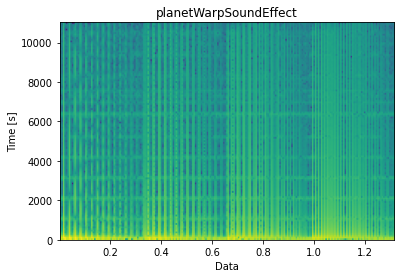
\includegraphics[width=6cm]{sound_effects/planetWarpSoundEffect.wav-spec.png}%
    } &
    \makecell[l]{
      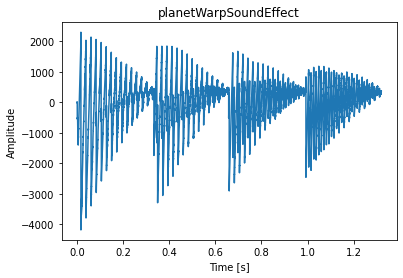
\includegraphics[width=6cm]{sound_effects/planetWarpSoundEffect.wav-amp.png}%
    } &
    \makecell[l]{
      \textattachfile{src/sound_effects/sounds/planetWarpSoundEffect.wav}{
\includegraphics[width=1cm]{sound_effects/sounds/play.png}}
    } \\
    \addlinespace
      \makecell[l]{
        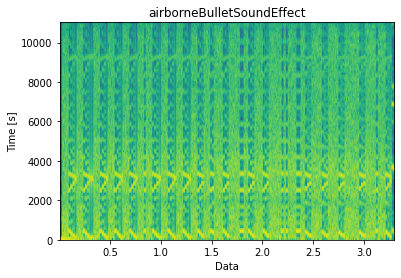
\includegraphics[width=6cm]{sound_effects/airborneBulletSoundEffect.wav-spec.png}%
      } &
    \makecell[l]{
      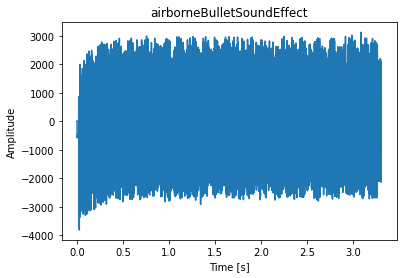
\includegraphics[width=6cm]{sound_effects/airborneBulletSoundEffect.wav-amp.png}%
    } &
    \makecell[l]{
      \textattachfile{src/sound_effects/sounds/airborneBulletSoundEffect.wav}{
\includegraphics[width=1cm]{sound_effects/sounds/play.png}}
    } \\
    \addlinespace
      \makecell[l]{
        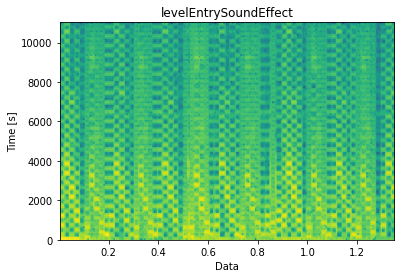
\includegraphics[width=6cm]{sound_effects/levelEntrySoundEffect.wav-spec.png}%
      } &
    \makecell[l]{
      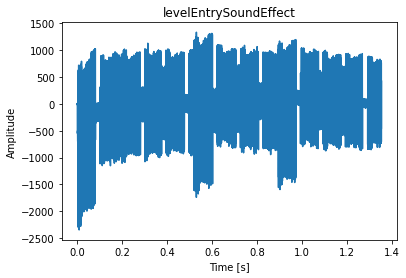
\includegraphics[width=6cm]{sound_effects/levelEntrySoundEffect.wav-amp.png}%
    } &
    \makecell[l]{
      \textattachfile{src/sound_effects/sounds/levelEntrySoundEffect.wav}{
\includegraphics[width=1cm]{sound_effects/sounds/play.png}}
    } \\
    \addlinespace
      \makecell[l]{
        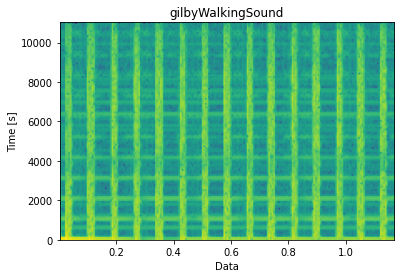
\includegraphics[width=6cm]{sound_effects/gilbyWalkingSound.wav-spec.png}%
      } &
    \makecell[l]{
      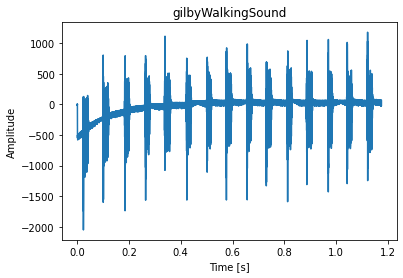
\includegraphics[width=6cm]{sound_effects/gilbyWalkingSound.wav-amp.png}%
    } &
    \makecell[l]{
      \textattachfile{src/sound_effects/sounds/gilbyWalkingSound.wav}{
\includegraphics[width=1cm]{sound_effects/sounds/play.png}}
    } \\
    \addlinespace
      \bottomrule
      \end{tabular}
    \end{adjustbox}
  }\caption{Some of the sound effects played during the game. On PDF viewers that support it, you can click the play icon to hear the effect.}
  \end{figure}
